\documentclass{VUMIFPSbakalaurinis}
\usepackage{algorithmicx}
\usepackage{algorithm}
\usepackage{algpseudocode}
\usepackage{amsfonts}
\usepackage{amsmath}
\usepackage{bm}
\usepackage{caption}
\usepackage{color}
\usepackage{float}
\usepackage{graphicx}
\usepackage{listings}
\usepackage{subfig}
\usepackage{wrapfig}
\usepackage{longtable}

% Titulinio aprašas
\university{Vilniaus universitetas}
\faculty{Matematikos ir informatikos fakultetas}
\department{Programų sistemų katedra}
\papertype{Bakalauro darbas}
\title{Paieškos proceso ir jos rezultatų pateikimo vartotojams panaudojamumas VUL Santaros klinikų svetainėje}
\titleineng{The Usability of the Search Process and Presenting its Results to the User for VUH Santaros Klinikos Website}
\author{Tomas Kiziela}
% \secondauthor{Vardonis Pavardonis}   % Pridėti antrą autorių
\supervisor{doc. Kristina Lapin}
\reviewer{}
\date{Vilnius – \the\year}

% Nustatymai
% \setmainfont{Palemonas}   % Pakeisti teksto šriftą į Palemonas (turi būti įdiegtas sistemoje)
\bibliography{bibliografija}

\begin{document}
\maketitle

% Padėkų skyrius
\sectionnonumnocontent{Padėkos asmenims ir organizacijoms}
\vspace{7cm}
\begin{center}
    
\end{center}

\sectionnonumnocontent{Santrauka}
%Glaustai aprašomas darbo turinys: pristatoma nagrinėta problema ir padarytos
%išvados. Santraukos apimtis ne didesnė nei 0,5 puslapio. Santraukų gale
%nurodomi darbo raktiniai žodžiai. 
% Nurodomi iki 5 svarbiausių temos raktinių žodžių (terminų).
% Vienas terminas gali susidėti iš kelių žodžių.
%\raktiniaizodziai{raktinis žodis 1, raktinis žodis 2, raktinis žodis 3, raktinis žodis 4, raktinis žodis 5}   

\sectionnonumnocontent{Summary}
%Santrauka anglų kalba. Santraukos apimtis ne didesnė nei 0,5 puslapio.
%\keywords{keyword 1, keyword 2, keyword 3, keyword 4, keyword 5}

\tableofcontents

\sectionnonum{Įvadas}
Šiame darbe tyrinėjami sprendimai Vilniaus Universiteto Ligoninės (VUL) Santaros klinikų tinklapio santa.lt panaudojamumo problemoms spręsti. Darbe buvo apibrėžti reikalavimai sistemai gauti iš naudotojų poreikių ir panaudojamumo analizės ir padaryti architektūriniai sprendimai. Šiame darbe yra remiamasi rezultatais iš autoriaus kursinio ir projektinio darbo ta pačia tema\cite{Kursinis, Projektinis}.

Autoriaus kursiniame darbe rasta, kad santa.lt tinklapio naudotojams yra aktualu rasti registraciją pas gydytoją ir ligoninės kontaktus, tačiau tinklapyje tai padaryti užtrunka ilgiau nei turėtų. Be šių problemų tinklapyje yra ir kitų panaudojamumo problemų rastų per panaudojamumo analizę. Tinklapio paieškos rezultatai neatitinka naudotojo įvestos užklausos, yra prastai surūšiuoti, filtravimas nėra efektyvus ir nėra patarimų kaip reikėtų teisingai naudoti paieškos sistemą. Navigacijos sistema turi per daug lygių ir yra nepakankamai plati, kategorijų pavadinimai neatitinka informacijos viduje ir puslapio elementai neteikia pakankamo atsako naudotojo veiksmams. Šiuos ir kitus rastus trūkumus ketinama ištaisyti galutinėje sistemoje.

Lietuva pagal 2018 metų DESI indeksą įvertinta 94 balais pagal plačiajuosčio ryšio kainą, 3 vieta Europos Sąjungoje (ES), o naujienas internetu skaito net 93\% gyventojų, daugiau nei bet kurioje kitoje ES valstybėje\cite{InternetasLt}. Iš to matosi, kad lietuviai turi prieinamą internetą ir dažnai jį pasitelkia kaip informacijos šaltinį. Technologiškai pažengusiose valstybėse su gerai išvystyta interneto infrastruktūra gyventojai dažnai ieško informacijos apie sveikatą internetu\cite{InternetUseByPublicSAEn}\cite{InternetUseByPublicHKEn}, tikėtina, kad tai galioja ir Lietuvoje.

VUL Santaros klinikos yra viena didžiausių Lietuvos ligoninių. Joje dirba virš 5000 darbuotojų ir kasmet gydoma apie milijonas pacientų\cite{VulSkApieMusLt}. Atrodo natūralu daryti prielaidą, kad nemažai pacientų ir lankytojų apie ligoninę domisi internetu ir ligoninei yra svarbu turėti tinklapį atitinkantį naudotojų lūkesčius.

Šio \textbf{darbo tikslas} yra apibrėžti reikalavimus ir projektavimo gaires sistemai, suprojektuoti puslapių architektūrą, navigacijos meniu ir pasirinkti serverio architektūros modelį. 

Uždaviniai:
\begin{enumerate}
	\item Identifikuoti reikalavimus sistemai
	\item Suprojektuoti tinklapį
\end{enumerate}

\sectionnonum{Panaudojamumo analizės rezultatai}
Kursiniame darbe buvo įvertintas esamo tinklapio panaudojamumas\cite{Kursinis} pagal David Travis gaires\cite{SearchGuidelinesEn}\cite{NavigationAndIAGuidelinesEn} ir Jakob Nielsen euristikas\cite{NielsenHeuristicsEn}. Prie defektų parašyti skaičiai nurodo kuris maketas (pav.) ir kuri maketo dalis (d.) juos taiso.

\begin{center}
\captionof{table}{Paieškos panaudojamumo gairių vertinimas pradiniam puslapiui}
\begin{tabular}{ |p{13cm}|p{2,5cm}| } 
 \hline
	Gairė & Ar tenkina? \\ \hline
	1) Pagrindinė paieška lengvai valdoma & tenkina \\ \hline
	2) Paieškos rezultatų puslapis naudotojui rodo, ko buvo ieškota, ir yra lengva pakeisti ir pakartoti užklausą & tenkina \\ \hline
	3) Paieškos rezultatai yra aiškūs, naudingi ir reitinguojami pagal atitikimą užklausai & ne (\ref{img:PaieškosPrototipas} pav. 2 d.) \\ \hline
	4) Paieškos rezultatų puslapis aiškiai parodo kiek rezultatų gražinta ir rezultatų skaičius per puslapį gali būti reguliuojamas naudotojo & tenkina \\ \hline
	5) Jei negražinamas nei vienas rezultatas, sistema pasiūlo idėjų ar nustatymų pagerinti užklausai atsižvelgiant į atpažįstamas įvesties problemas & ne (\ref{img:PaieškosPrototipas} pav. 4 d.) \\ \hline
	6) Paieška dailiai susitvarko su tuščia užklausa & tenkina \\ \hline
	7) Dažniausios užklausos gražina naudingus rezultatus & ne (\ref{img:PaieškosPrototipas} pav. 2 d.) \\ \hline
	8) Paieškos sistema turi šabloną arba patarimus kaip ją deramai naudoti & ne (\ref{img:PaieškosPrototipas} pav. 4 d.) \\ \hline
	9) Puslapis turi pajėgesnę paieškos sąsają leidžiančią naudotojams patikslinti užklausas & tenkina \\ \hline
	10) Paieškos rezultatų puslapis nerodo besikartojančių rezultatų & tenkina \\ \hline
	11) Paieškos laukas pakankamai ilgas dažniausių užklausų ilgiams & ne (\ref{img:PaieškosPrototipas} pav. 1 d.) \\ \hline
	12) Paieška apima visą interneto svetainę, o ne tik jos dalį & tenkina \\ \hline
	13) Jei svetainė leidžia naudotojams sudaryti sudėtingą paiešką, šios paieškos gali būti išsaugojamos ir kartojamos reguliariai & tenkina \\ \hline
	14) Paieškos sąsaja padėta, naudotojams įprastoje vietoje (viršuje dešinėje) & tenkina \\ \hline
	15) Paieškos laukas ir jo kontrolės aiškiai pavadintos & tenkina \\ \hline
	16) Puslapis palaiko paieškos strategiją ir naršymo strategiją & ne (\ref{img:PaieškosPrototipas} pav.) \\ \hline
	17) Paieškos sritis aiškiai parašyta paieškos rezultatų puslapyje ir naudotojai gali ją susiaurinti & tenkina \\ \hline
	18) Paieškos rezultatų puslapis atvaizduoja naudingą meta informaciją (informacija apie informaciją), kaip dokumento dydis, dokumento sukūrimo data ir failo tipas & tenkina \\ \hline
	19) Paieškos sistema automatiškai patikrina rašybą ir ieško daugiaskaitinių formų ir sinonimų & ne \\ \hline
	20) Paieškos sistema leidžia ieškoti panašių rezultatų („daugiau tokių“) & ne (\ref{img:PaieškosPrototipas} pav. 5 d.) \\ \hline
\end{tabular}
\label{PaieškosLentelėPrad}
\end{center}
\pagebreak


\captionof{table}{Navigacijos ir informacijos architektūros panaudojamumo gairių vertinimas}
\begin{longtable}{ |p{12,6cm}|p{2,9cm}| } 
 \hline
	Gairė & Ar tenkina? \\ \hline
	1) Yra patogus ir akivaizdus būdas judėti tarp susijusių puslapių ir skyrių ir yra lengva grįžti į pagrindinį puslapį & tenkina \\ \hline
	2) Informacija, kurios naudotojams dažnai prireikia yra lengvai pasiekiama iš daugumos puslapių & tenkina \\ \hline
	3) Navigacijos pasirinkimai išrikiuoti pačiu racionaliausiu arba užduočiai orientuotu būdu & tenkina \\ \hline
	4) Navigacijos sistema plati ir sekli (daug meniu elementų), o ne gili (daug meniu lygių)  & ne (\ref{img:NavigacijosPrototipas} pav. 4, 6 d.) \\ \hline
	5) Paprasta, aiškaus modelio svetainės struktūra be nereikalingų lygių & ne (\ref{img:NavigacijosPrototipas} pav. 4, 6 d.) \\ \hline
	6) Pagrindiniai puslapio skyriai pasiekiami iš bet kurio puslapio ir nėra aklaviečių & tenkina \\ \hline
	7) Navigacijos skirtukai patalpinti puslapio viršuje ir atrodo kaip paspaudžiamos versijos realaus pasaulio skirtukų & ne \\ \hline
	8) Yra svetainės žemėlapis, kuris suteikia svetainės turinio apžvalgą & tenkina \\ \hline
	9) Svetainės žemėlapį galima pasiekti iš bet kurio puslapio & tenkina \\ \hline
	10) Svetainės žemėlapis suteikia glaustą svetainės apžvalgą, o ne pernaudotą navigacijos meniu ar sąrašą kiekvienos temos & ne \\ \hline
	11) Suteikiamas geras navigacijos grįžtamasis ryšys (rodoma, kur randiesi puslapyje) & tenkina \\ \hline
	12) Kategorijų pavadinimai tiksliai apibūdina informaciją viduje & ne (\ref{img:NavigacijosPrototipas} pav. 4, 6 d.) \\ \hline
	13) Nuorodos ir navigacijos pavadinimai susidaro iš raktinių žodžių, kurių naudotojai ieškos bandydami atlikti užduotį & tenkina \\ \hline
	14) Terminologija ir susitarimai (kaip nuorodų spalvos) (maždaug) atitinka bendrą interneto naudojimą & tenkina \\ \hline
	15) Nuorodos atrodo taip pačiai skirtingose svetainės dalyse & tenkina \\ \hline
	16) Navigacijos elementams ir hiperteksto nuorodoms naudojami terminai yra nedviprasmiški ir be žargono & tenkina \\ \hline
	17) Matomi pasikeitimai, kai naudotojas užveda kursorių ant kažko paspaudžiamo (neįskaitant kursoriaus pasikeitimų) & ne (\ref{img:NavigacijosPrototipas} pav. 4, 6 d.) \\ \hline
	18) Svarbus turinys pasiekiamas iš daugiau nei vienos nuorodos (naudotojams gali reikėt skirtingų nuorodų pavadinimų) & tenkina \\ \hline
	19) Puslapiai skirti tik navigacijai (pavyzdžiui pradinis puslapis) gali būti peržiūrimi be slinkimo & tenkina \\ \hline
	20) Svetainė leidžia naudotojui kontroliuoti sąveikos greitį ir eiliškumą & tenkina \\ \hline
	21) Visuose puslapiuose yra aiškiai pažymėti išėjimai leidžiantys naudotojui pabėgti iš esamos užduoties be papildomo dialogo & tenkina \\ \hline
	22) Svetainė neišjungia naršyklės „atgal“ mygtuko ir „atgal“ mygtukas visada matomas naršyklės įrankių juostoje & tenkina \\ \hline
	23) Paspaudus „atgal“ mygtuką naudotojas visada gražinamas į puslapį, iš kurio atėjo & tenkina \\ \hline
	24) Jeigu puslapis sukuria naujus langus, jie neklaidina naudotojo (jie dialogo lango dydžio ir lengvai uždaromi) & tenkina \\ \hline
	25) Meniu instrukcijos, nurodymai ir žinutės atsiranda toje pačioje vietoje visuose puslapiuose & tenkina \\ \hline
\end{longtable}
\label{NavigacijosirIALentelėPrad}
\addtocounter{table}{-1}
\setlength{\parindent}{1cm}

\begin{center}
\captionof{table}{Euristinis vertinimas, DS - defekto sunkumas}
\begin{tabular}{ | p{3,6cm} | p{0,3cm} | p{11,6cm} | } 
 \hline
	Euristika & DS & Komentaras \\ \hline
	1) Sistemos būsenos matomumas & 2 & Paspaudus mygtuką „ieškoti“ rodomas tuščias puslapis iki paieškos rezultatų gavimo. Paieška užtrunka apie 3 sekundes, taigi galėtų būti tekstas, animacija ar progreso juosta pranešanti, kad vyksta paieška. Užvedus kursorių ant paspaudžiamų elementų kaip nuorodų ir tam tikrų elementų, šie nepasikeičia, taigi vartotojui sunkiau juos pastebėti. \\ \hline
	2) Atitikimas realiam pasauliui  & 2 & Daugumai vartotojų aktuali registracija pas gydytoją, taigi ji turėtų būti dar lengviau surandama naršant arba ieškant. (\ref{img:NavigacijosPrototipas} pav. 2 d.) \\ \hline
	3) Naudotojo valdomas dialogas & 1 & Dalis puslapių nerodo nukeliauto kelio, kai šie randami per paiešką. (\ref{img:NavigacijosPrototipas} pav. 3 d.) \\ \hline
	4) Darna ir standartai & 1 & Kai kuriuose puslapiuose pranyksta navigacijos elementai. \\ \hline
	5) Klaidų prevencija & 2 & Netinkami numatytieji nustatymai lemia, kad naudotojai dažnai atlieka netinkamą paiešką. Nėra patarimų kaip naudotis paieškos sistema. Vedant užklausą nepasiūlomi paieškos variantai. (\ref{img:PaieškosPrototipas} pav. 2, 4 d.) \\ \hline
	6) Atpažinimas geriau nei atsiminimas & 2 & Navigacija nerodo gilesnių lygių, kol neatidaromas to lygio puslapis, taigi reikia žinoti, kurioje kategorije ieškomas elementas. Trūksta vaizdų, kurie asocijuojasi su mygtukais. Nėra pagalbos naudotis tinklapiu. (\ref{img:NavigacijosPrototipas} pav. 6, 5, 1 d.) \\ \hline
	7) Naudojimo lankstumas ir našumas & 2 & Nerodomi susiję puslapiai. Negalima nueiti į giliausią kategorijos lygį vienu paspaudimu, reikia eiti per tėvinius elementus. (\ref{img:NavigacijosPrototipas} pav. 6 d.) \\ \hline
	8) Estetiškas ir minimalistinis dizainas & 2 & Pertekliniai paspaudimai bandant naviguoti per kategorijas. (\ref{img:NavigacijosPrototipas} pav. 6 d.) \\ \hline
	9) Remti klaidų atpažinimą, jų priežasčių nustatymą ir taisymą & 0 &  \\ \hline
	10) Parama ir dokumentacija & 2 & Nėra informacijos ar pavyzdžių kaip naudoti sudėtingas paieškos funkcijas. (\ref{img:PaieškosPrototipas} pav. 4 d.) \\ \hline
\end{tabular}
\label{EuristikųLentelėPrad}
\end{center}

\sectionnonum{Sprendimo maketai}
Kursiniame darbe gauti maketai nurodantys pakeitimus paieškos sistemai ir informacijos architektūrai.

\begin{figure}[H]
    \centering
    \includegraphics[scale=0.65]{img/PaieškosPrototipas}
    \caption{Paieškos sistemos maketas su pataisymais}
    \label{img:PaieškosPrototipas}
\end{figure}

\begin{figure}[H]
    \centering
    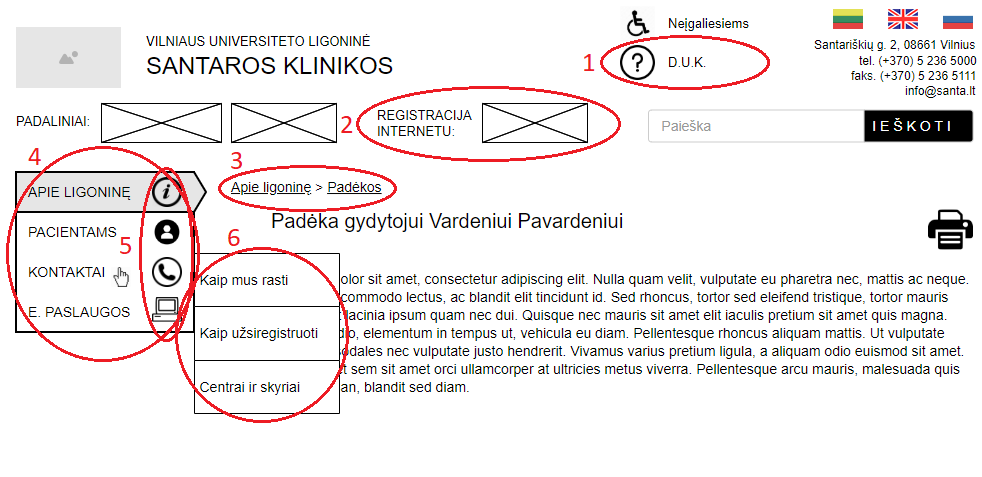
\includegraphics[scale=0.65]{img/NavigacijosPrototipas}
    \caption{Navigacijos sistemos maketas su pataisymais}
    \label{img:NavigacijosPrototipas}
\end{figure}




\sectionnonum{Rezultatai ir išvados}
%Šiame darbe išskirti funkciniai ir nefunkciniai reikalavimai paieškai, navigacijos ir informacijos architektūros projektavimo gairės, parinkti tinklapio architektūros maketai, suprojektuotas navigacijos meniu ir aprašytas bendras sistemos serverio architektūros modelis.

%Formuluojant reikalavimus iš gairių autorius pastebėjo, kad nevisiems defektams prasminga rašyti reikalavimus, kadangi nevisi defektai yra aktualūs gerinamai sistemai, o kai kurie turi bendrą iškilimo priežastį. Atliekant vertikalios ir horizontalios navigacijos palyginimą išsiaiškinta, kad vertikali geriau tinka, kai meniu labai platus ir yra naudojamas kaip orientacinis elementas, ne tik informacijos paieškos elementas. Taip pat paaiškėjo, kad horizontalų meniu gerai naudoti, kai kažkurie skyriai daug dažniau naudojami, ir jį naudojant galima užimti mažiau vietos navigacijai. Projektuojant navigacijos meniu autorius pastebėjo, kad net sutalpinus daug skyrių į meniu, informacija gali būti lengvai surandama, jeigu viskas tvarkingai surūšiuota.

%Rezultatų ir išvadų dalyje turi būti aiškiai išdėstomi pagrindiniai darbo
%rezultatai (kažkas išanalizuota, kažkas sukurta, kažkas įdiegta) ir pateikiamos
%išvados (daromi nagrinėtų problemų sprendimo metodų palyginimai, teikiamos
%rekomendacijos, akcentuojamos naujovės).

\printbibliography[heading=bibintoc, title=Šaltiniai]  % Šaltinių sąraše nurodoma panaudota
% literatūra, kitokie šaltiniai. Abėcėlės tvarka išdėstomi darbe panaudotų
% (cituotų, perfrazuotų ar bent paminėtų) mokslo leidinių, kitokių publikacijų
% bibliografiniai aprašai. Šaltinių sąrašas spausdinamas iš naujo puslapio.
% Aprašai pateikiami netransliteruoti. Šaltinių sąraše negali būti tokių
% šaltinių, kurie nebuvo paminėti tekste. Šaltinių sąraše rekomenduojame
% necituoti savo kursinio darbo, nes tai nėra oficialus literatūros šaltinis.
% Jei tokių nuorodų reikia, pateikti jas tekste.

% \sectionnonum{Sąvokų apibrėžimai}
%\sectionnonum{Santrumpos}
%Sąvokų apibrėžimai ir santrumpų sąrašas sudaromas tada, kai darbo tekste
%vartojami specialūs paaiškinimo reikalaujantys terminai ir rečiau sutinkamos
%santrumpos.

\appendix  % Priedai
% Prieduose gali būti pateikiama pagalbinė, ypač darbo autoriaus savarankiškai
% parengta, medžiaga. Savarankiški priedai gali būti pateikiami ir
% kompaktiniame diske. Priedai taip pat numeruojami ir vadinami. Darbo tekstas
% su priedais susiejamas nuorodomis.
\sectionnonum{Trys puslapių tipai}

\begin{figure}[H]
    \centering
    
\includegraphics[scale=0.65]{img/Pagrindinis}
    \caption{Pagrindinis puslapis}
    \label{img:PagrindinisPuslapis}
\end{figure}
\begin{figure}[H]
    \centering
    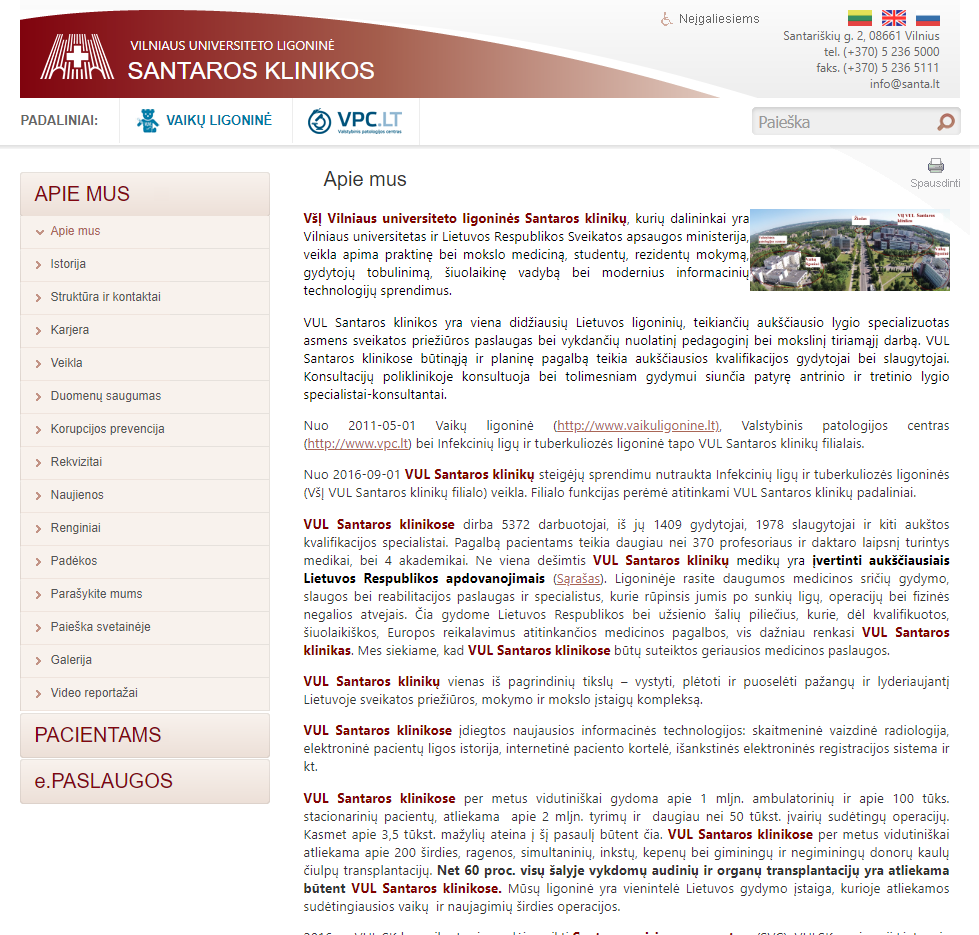
\includegraphics[scale=0.65]{img/Turinys}
    \caption{Turinio puslapis}
    \label{img:TurinysPuslapis}
\end{figure}
\begin{figure}[H]
    \centering
    \includegraphics[scale=0.65]{img/Paieška}
    \caption{Paieškos puslapis}
    \label{img:PaieškaPuslapis}
\end{figure}


%\section{Eksperimentinio palyginimo rezultatai}
% tablesgenerator.com - converts calculators (e.g. excel) tables to LaTeX
%\begin{table}[H]\footnotesize
%  \centering
%  \caption{Lentelės pavyzdys}
%  {\begin{tabular}{|l|c|c|} \hline
%    Algoritmas & $\bar{x}$ & $\sigma^{2}$ \\
%    \hline
%    Algoritmas A  & 1.6335    & 0.5584       \\
%    Algoritmas B  & 1.7395    & 0.5647       \\
%    \hline
%  \end{tabular}}
%  \label{tab:table example}
%\end{table}

\end{document}
